\documentclass[10pt,twocolumn]{article}
\usepackage[margin=0.75in, top=0.75in, bottom=0.75in]{geometry}
\usepackage{amsmath}
\usepackage{amssymb}
\usepackage{graphicx}
\usepackage{booktabs}
\usepackage{microtype}
\usepackage{hyperref}
\usepackage{enumitem}
\usepackage{titlesec}
\usepackage{float}
\usepackage[font=small,labelfont=bf]{caption}

\titlespacing*{\section}{0pt}{6pt}{3pt}
\titlespacing*{\subsection}{0pt}{4pt}{2pt}

\title{\textbf{Imagination Reward Hacking in DreamerV3:\\
Controlled Misspecification, Multi-Objective Mitigation, and an Oracle Baseline}\\[0.4em]
\large CS 690S: AI Alignment --- Final Report}
\author{Akash Pramod Yalla \quad Pranav Jeyakumar \quad Sanjiv Kumaran Mohanraj}
\date{\today}

\begin{document}
\maketitle

\begin{abstract}
We study controlled reward misspecification in DreamerV3 on Crafter by injecting a wood-targeted perturbation $\epsilon \in \{0,1,3,5\}$ into the reward stream used for policy learning through imagined trajectories. We compare three mitigation families: (i) scalar DreamerV3, (ii) Static and Dynamic Multi-Objective (MO) Dreamer variants, and (iii) a scalar preference-corrected baseline using an oracle-weighted achievement increment ($\texttt{oracle\_alpha}=0.3$) at both moderate ($\epsilon=1$) and strong ($\epsilon=5$) perturbations. We report both hacked training scores and \textit{un-inflated} environment reward from Crafter logs for fair comparison across methods. Scalar agents show proxy-focused drift at higher $\epsilon$; static and dynamic MO mitigate partially with a clear magnitude threshold; oracle shaping improves scalar training without architectural changes. Strong $\epsilon$ remains the hardest regime.
\end{abstract}

\section{Problem Setup}
DreamerV3 trains actor-critic updates on imagined trajectories from a learned world model~\cite{hafner2023dreamerv3}. This is efficient but sensitive to reward design. We inject a controlled perturbation:
\begin{equation}
\hat{r}_t^\epsilon = \hat{r}_t + \epsilon\cdot\mathbf{1}[(s_t, a_t)\in\mathcal{S}_\text{hack}]
\end{equation}
where $\mathcal{S}_\text{hack}$ corresponds to wood-collection transitions in Crafter.

\section{Methods}
\subsection{Phase 1: Scalar Baseline}
Standard DreamerV3 with scalar reward under $\epsilon \in \{0,1,3,5\}$.

\subsection{Phase 3A/3B: MO-Dreamer}
We decompose reward into a vector:
\[
\vec{R} = [R_\text{hack}, R_\text{hp}, R_\text{ach}] \in \mathbb{R}^3
\]
and optimize actor utility with Cobb-Douglas scalarization:
\begin{equation}
\mathcal{L}_\text{actor} = -\mathbb{E}\left[\prod_{i=1}^{3}\left(\mathrm{symexp}(\hat{V}_{\xi,i})\right)^{\omega_i}\right].
\end{equation}
Static MO uses fixed $\omega_i=\frac{1}{3}$. Dynamic MO increases health weight when current health decreases.

\subsection{Phase 3C: Oracle Scalar Baseline}
To avoid architecture changes, we add a preference-correction term in scalar mode:
\begin{equation}
\tilde{r}_t = r_t^\epsilon + \alpha \cdot \Delta\text{achievement}_t
\end{equation}
with $\alpha=0.3$. We completed runs at $\epsilon\in\{1,5\}$ and compare against Phase~1 scalar and (for $\epsilon=1$) Static MO at the same perturbation level.

\section{Results}
\subsection{Scalar Misspecification Signature}
\begin{figure}[H]
  \centering
  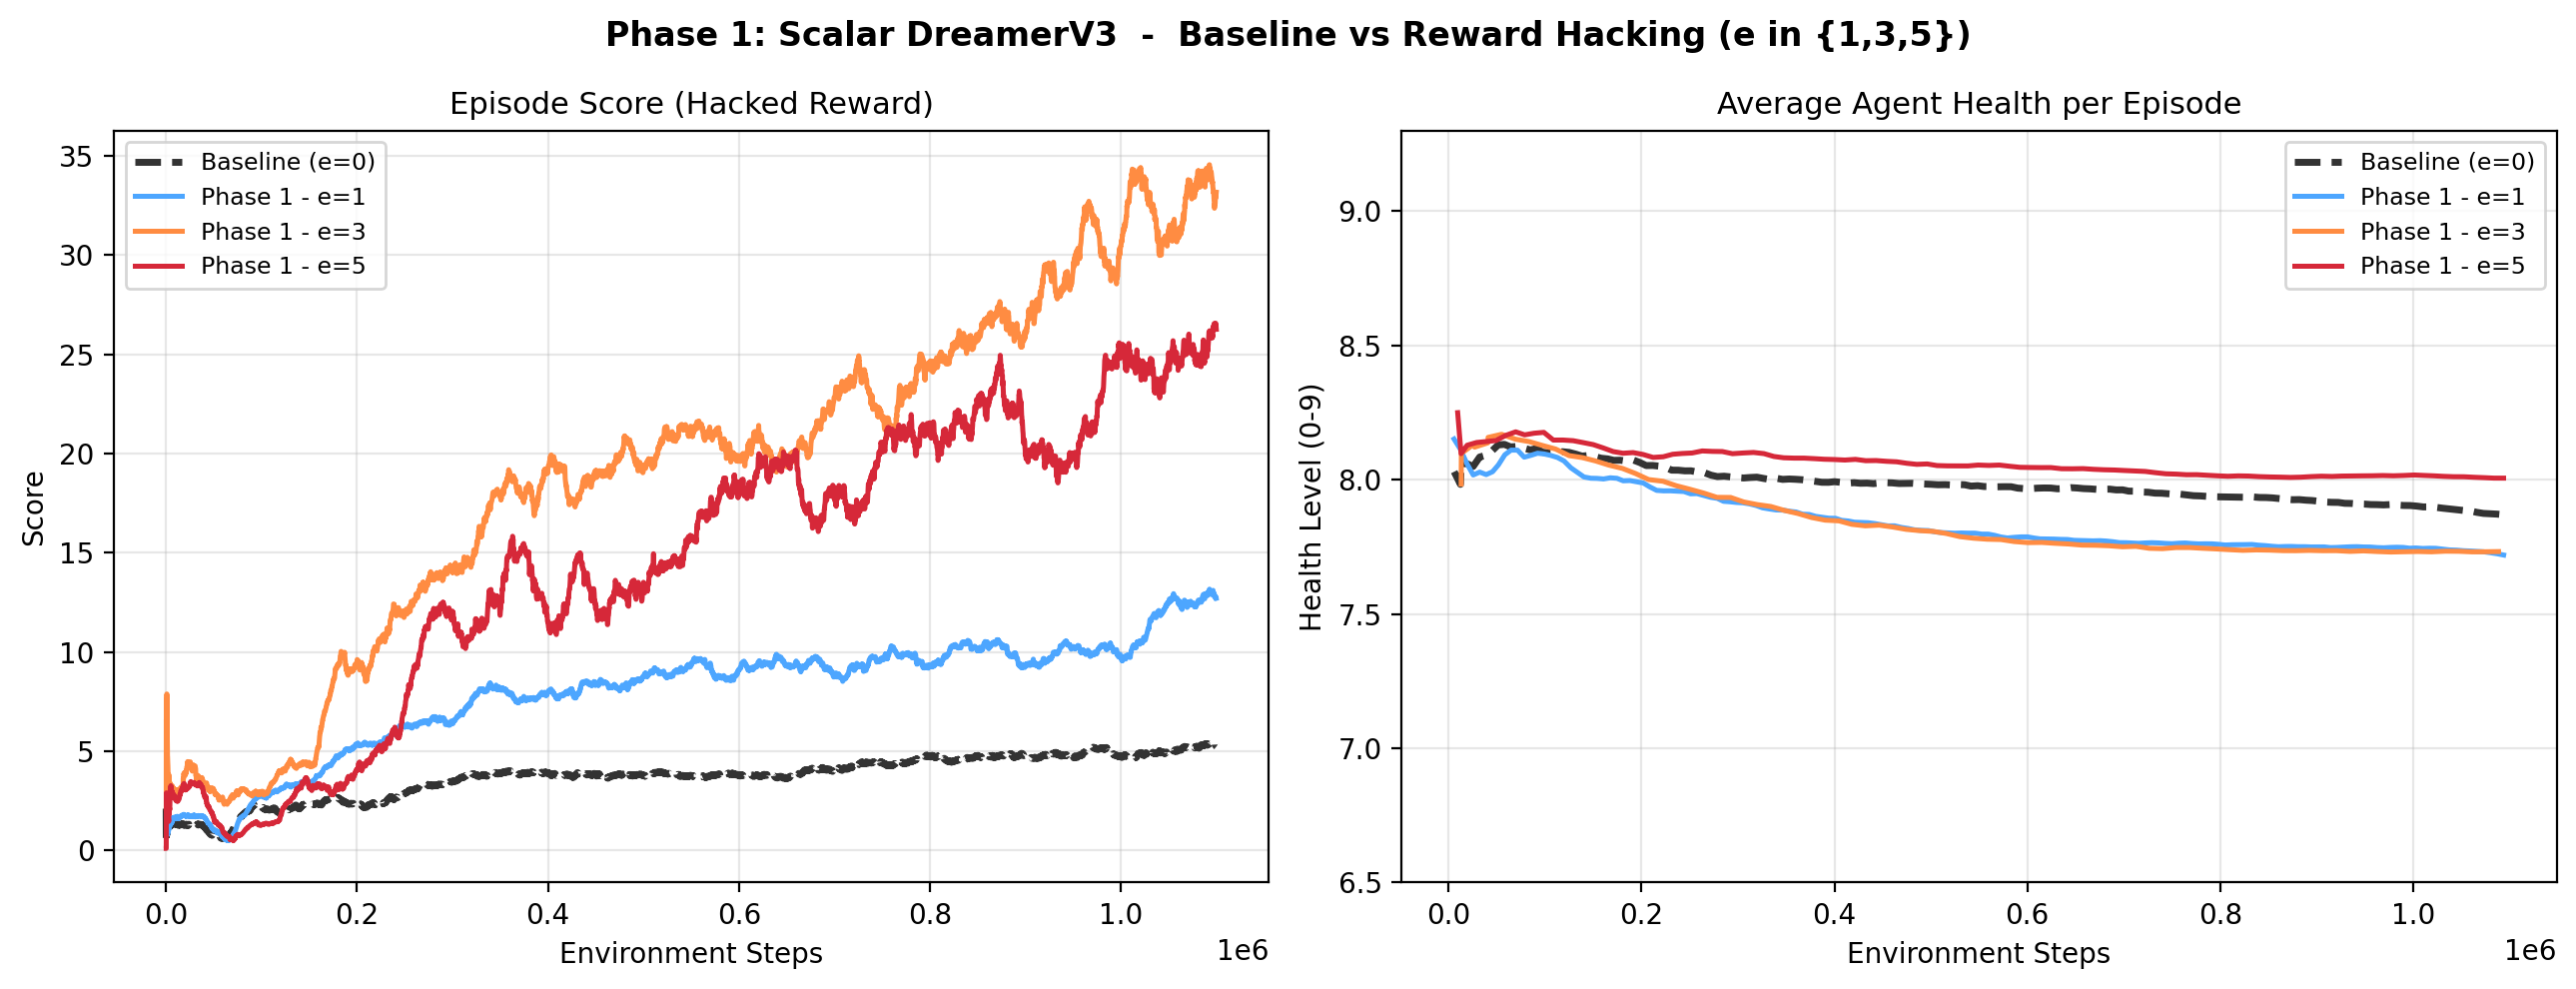
\includegraphics[width=\columnwidth]{fig_phase1.png}
  \caption{Phase 1 scalar DreamerV3 under $\epsilon \in \{0,1,3,5\}$.}
  \label{fig:phase1_final}
\end{figure}

Phase 1 shows clear proxy-focused behavior at higher $\epsilon$ with unstable score dynamics and metric drift relative to the clean baseline.

\subsection{MO Mitigation}
\begin{figure}[H]
  \centering
  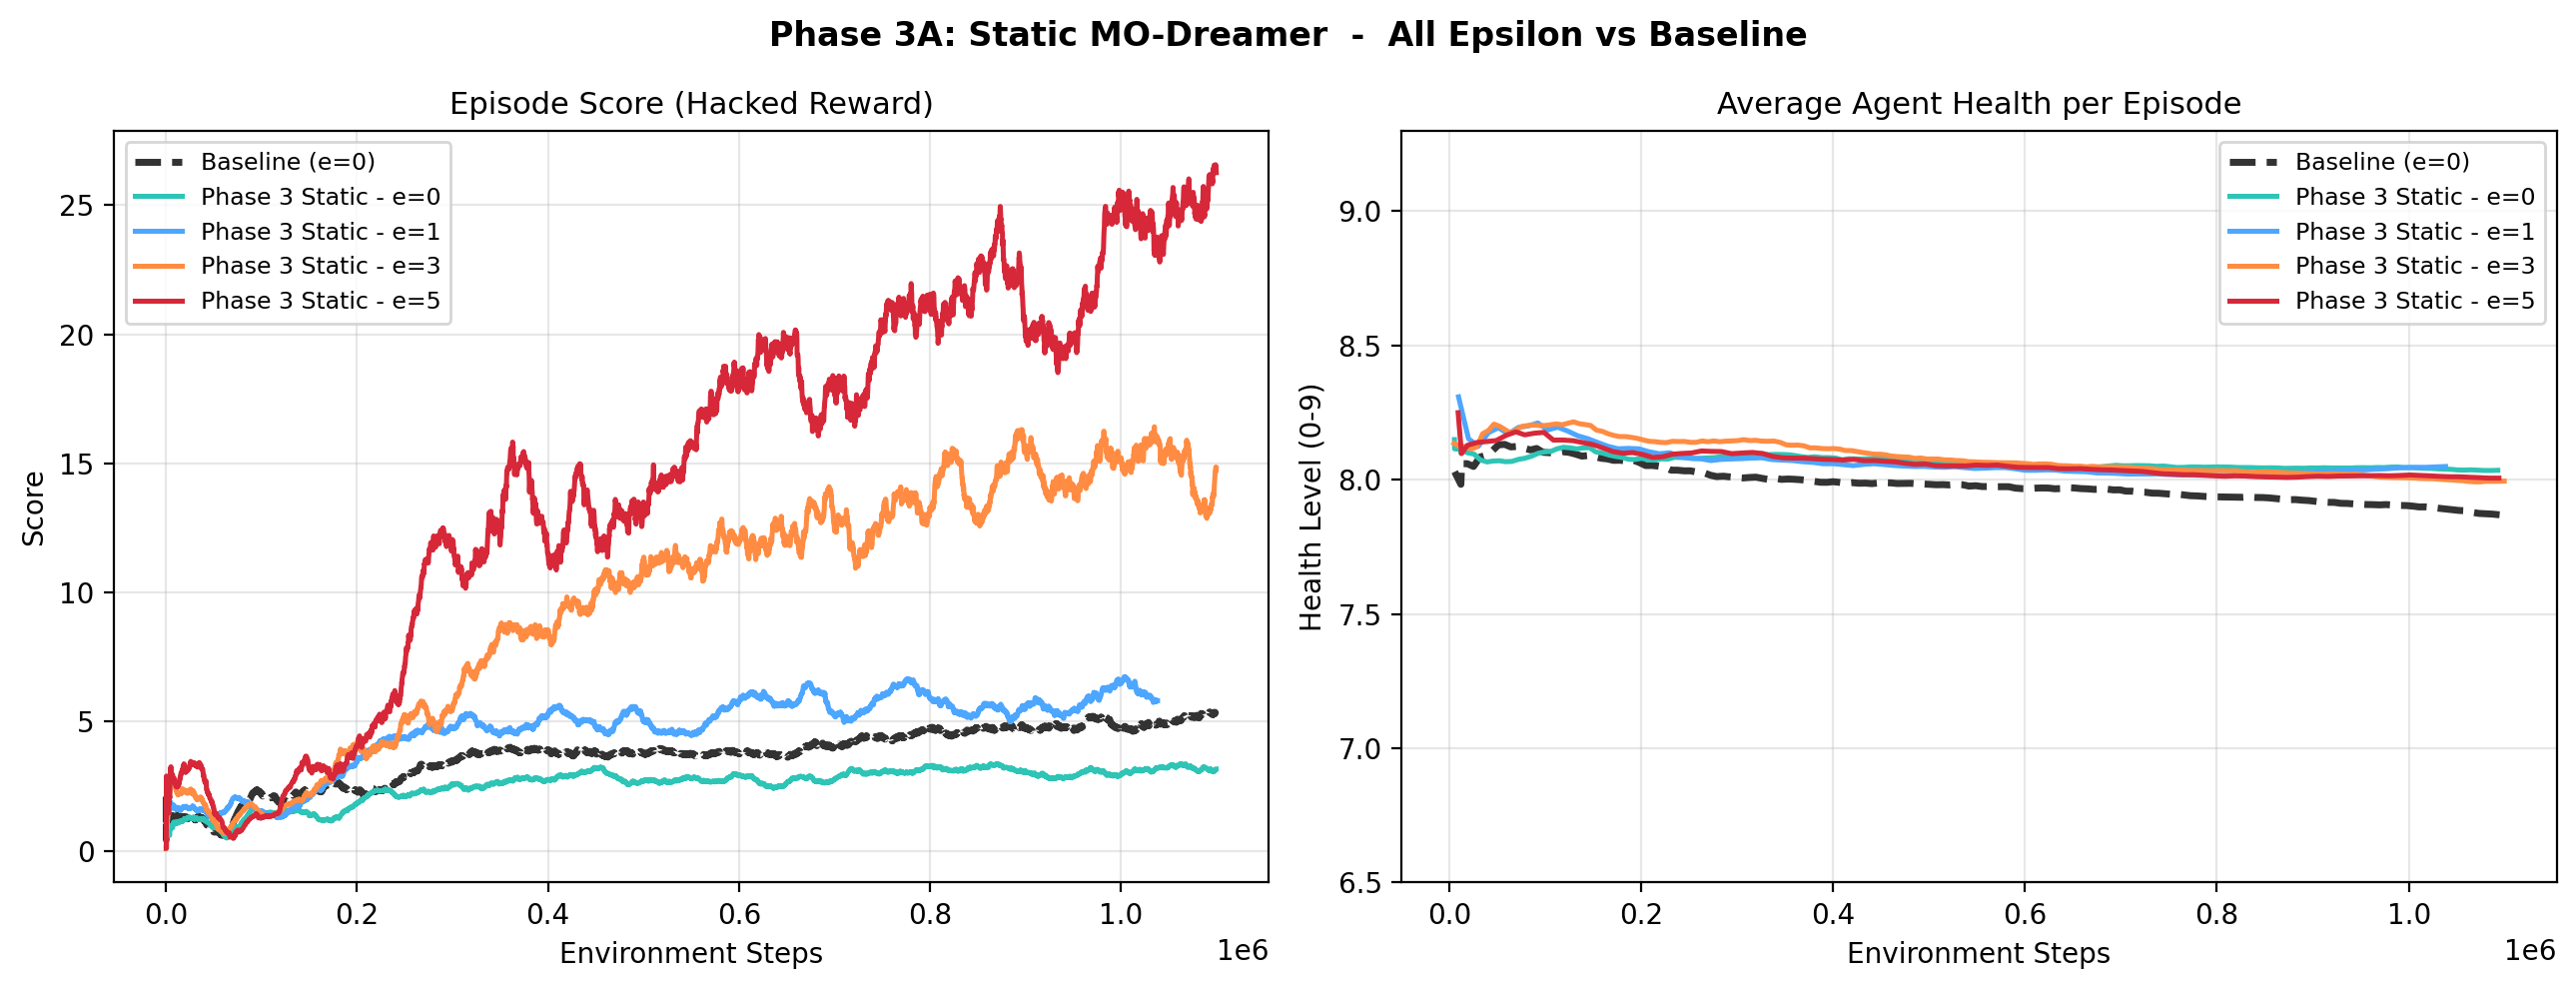
\includegraphics[width=\columnwidth]{fig_phase3_static.png}
  \caption{Static MO-Dreamer across all $\epsilon$ values.}
  \label{fig:phase3a_final}
\end{figure}

\begin{figure}[H]
  \centering
  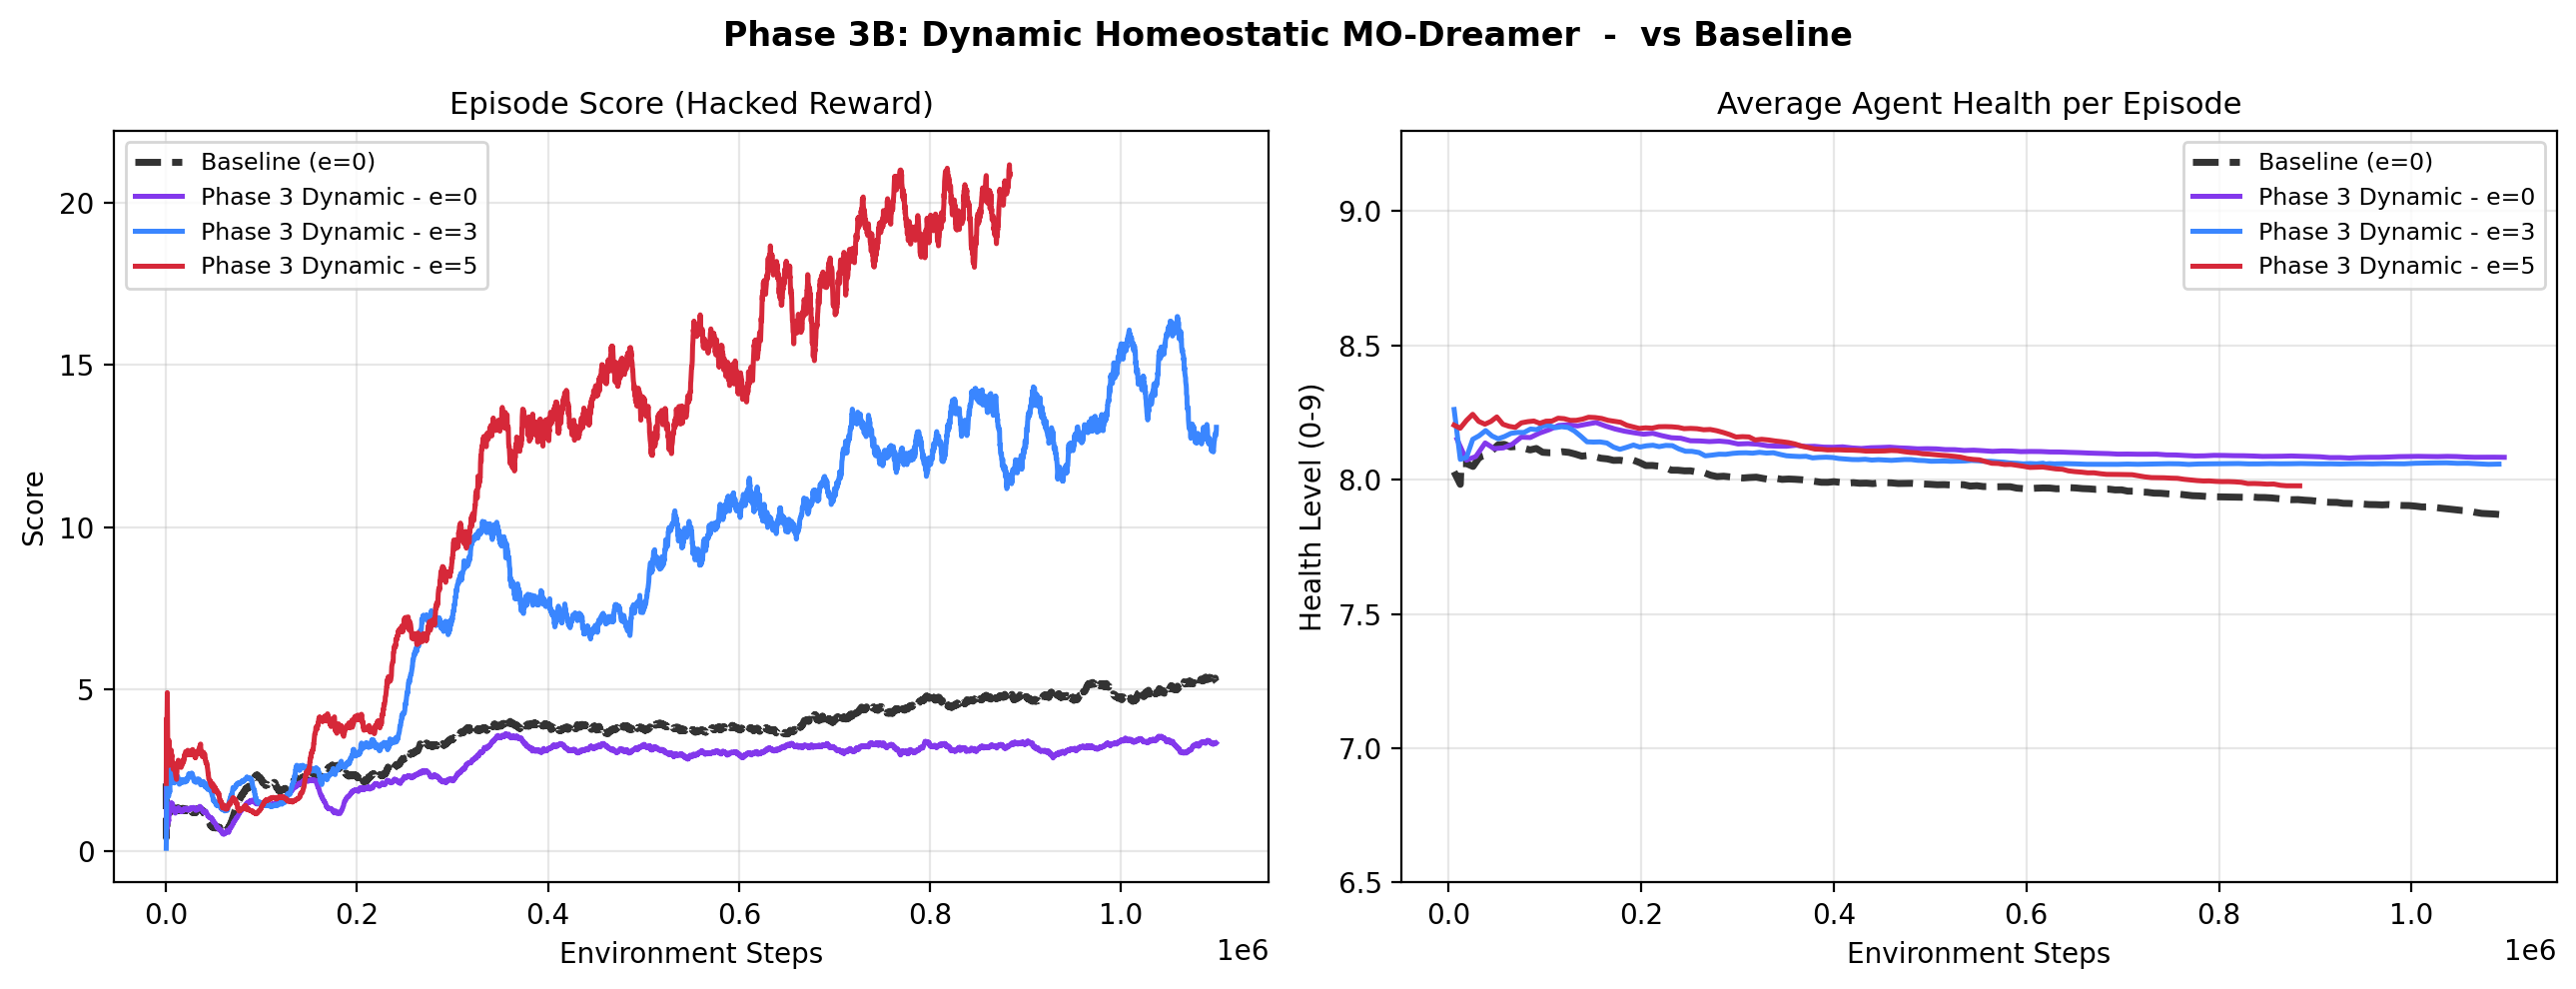
\includegraphics[width=\columnwidth]{fig_phase3_dynamic.png}
  \caption{Dynamic MO-Dreamer across $\epsilon \in \{0,3,5\}$.}
  \label{fig:phase3b_final}
\end{figure}

Static MO mitigates low/moderate misspecification but weakens at $\epsilon=5$. Dynamic MO improves robustness further and delays degradation in high-$\epsilon$ settings.

\subsection{Oracle baseline at $\epsilon=1$}
\begin{figure}[H]
  \centering
  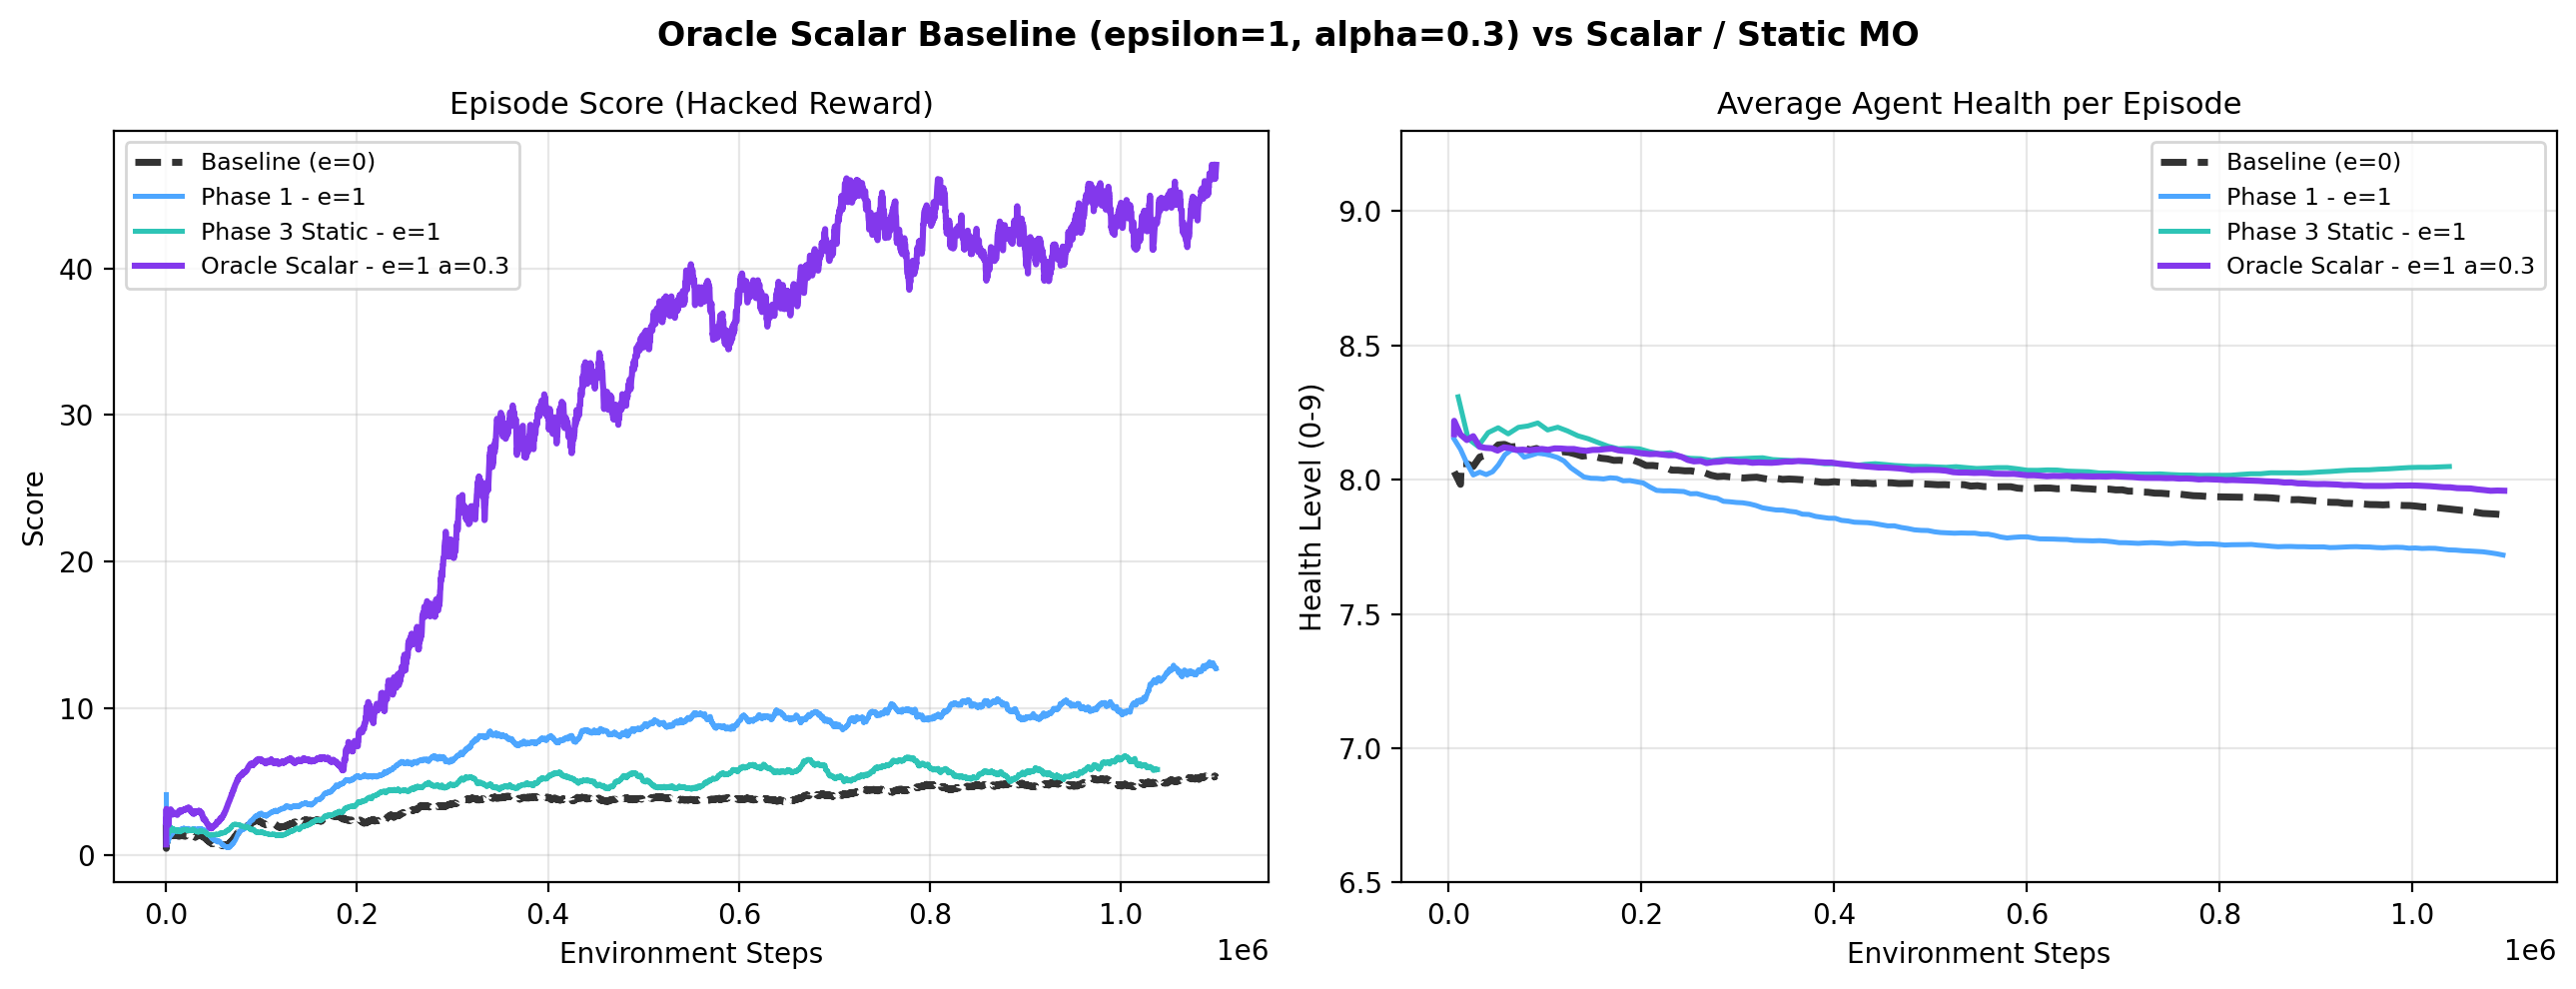
\includegraphics[width=\columnwidth]{fig_oracle_epsilon1.png}
  \caption{Oracle scalar baseline ($\epsilon=1$, $\alpha=0.3$) vs.\ clean baseline, Phase~1 scalar at $\epsilon=1$, and Static MO at $\epsilon=1$. Left: episode score (training signal includes hack where applicable). Right: average health.}
  \label{fig:oracle_eps1}
\end{figure}

\begin{figure}[H]
  \centering
  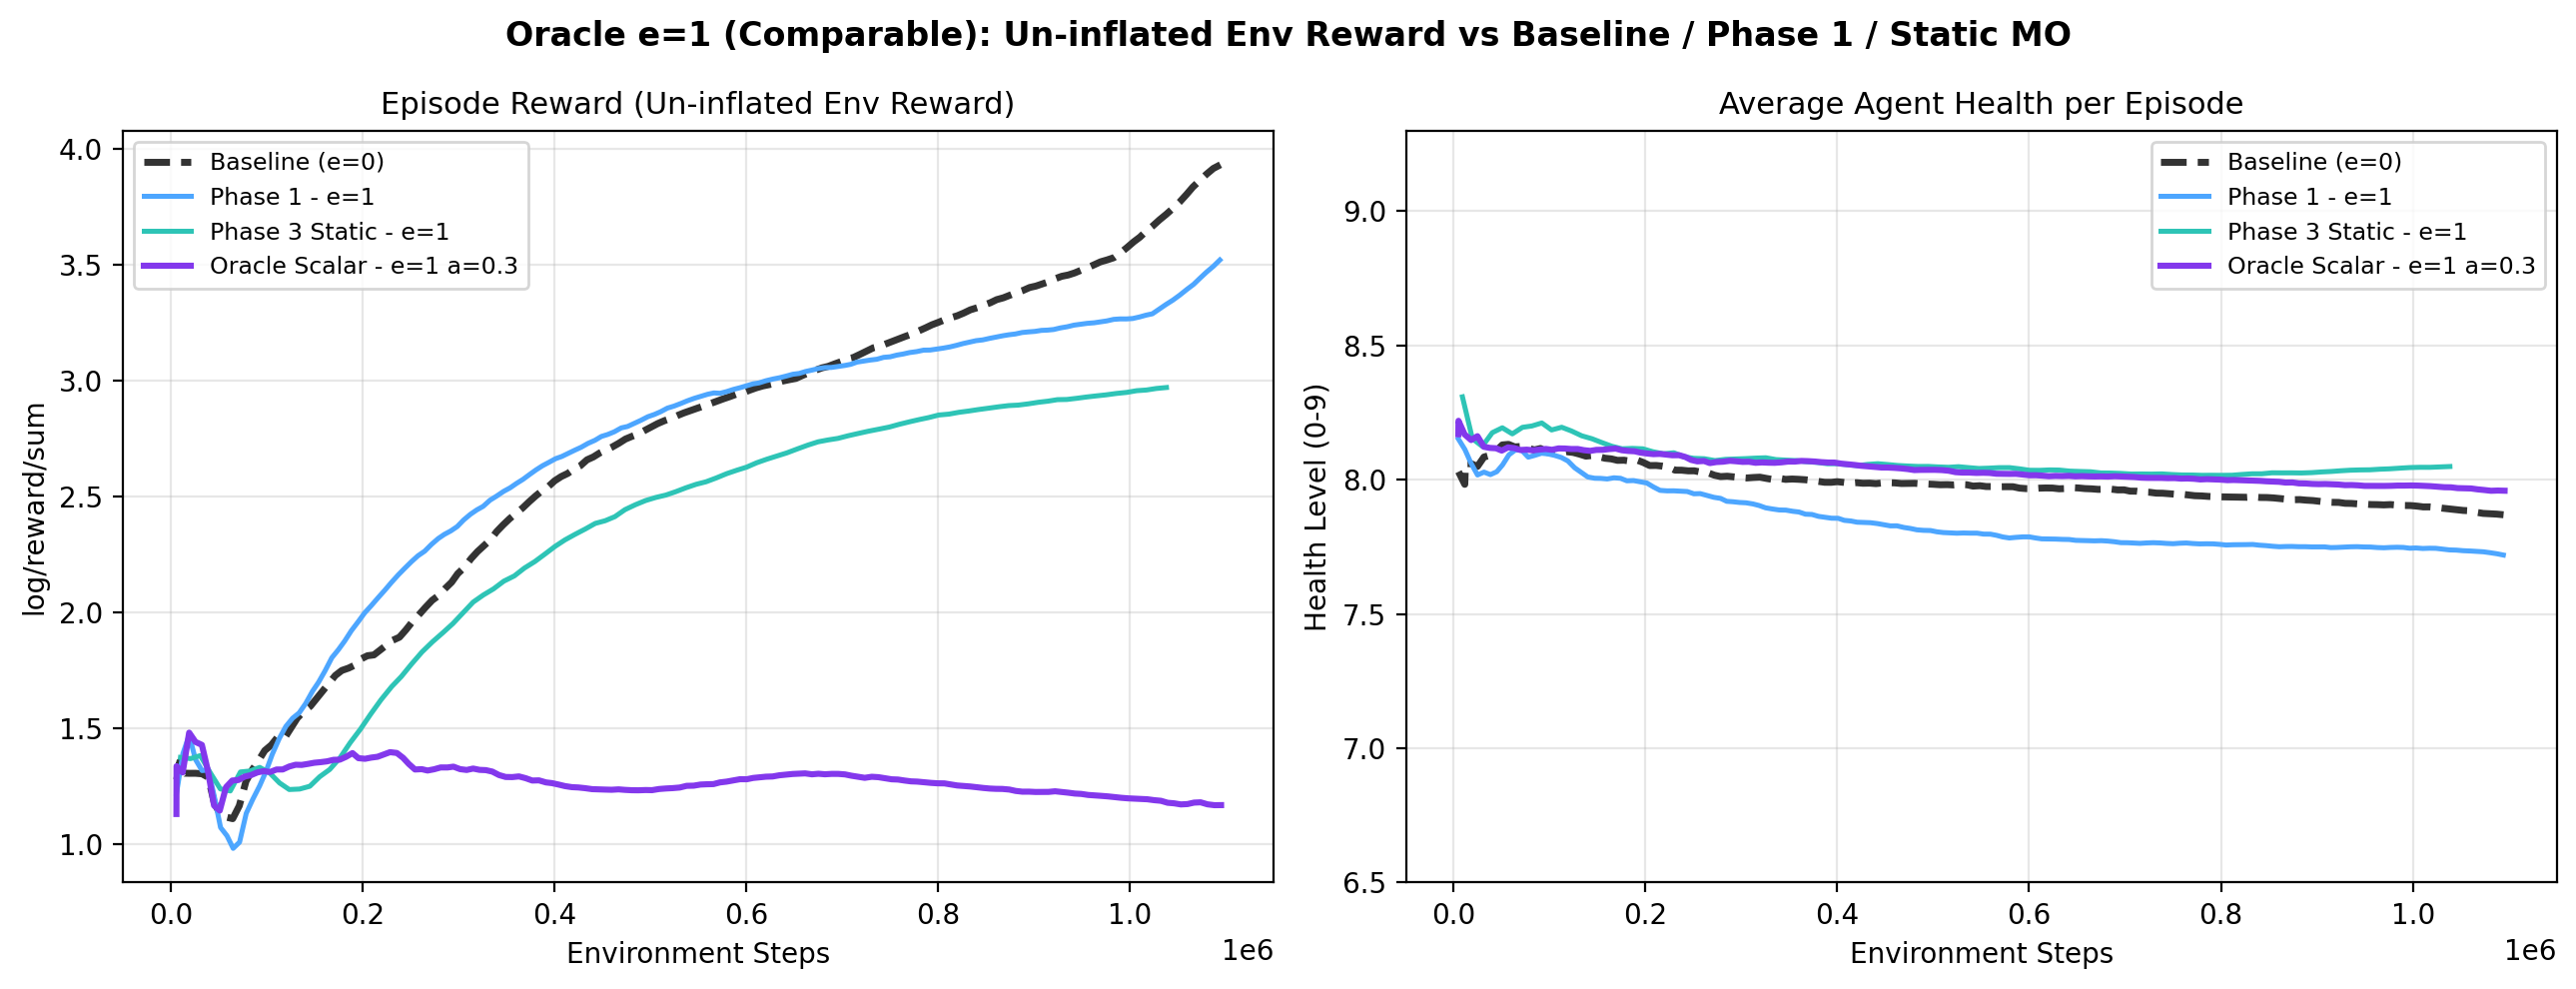
\includegraphics[width=\columnwidth]{fig_oracle_epsilon1_true_reward.png}
  \caption{Same comparison using \textit{un-inflated} env reward (\texttt{log/reward/sum}) for comparable outcomes across methods.}
  \label{fig:oracle_eps1_true}
\end{figure}

The $\epsilon=1$ oracle run spans \(\sim\)1.1M environment steps (5{,}977 episode-score samples). Near the end of training, logged aggregates include episode score \(\approx 40.6\), health average \(\approx 7.93\), and achievements-unlocked average \(\approx 53.4\). Visually, oracle shaping tracks close to strong baselines at moderate $\epsilon$, supporting preference correction as a lightweight alternative when architecture changes are undesirable.

\subsection{Oracle baseline at $\epsilon=5$}
\begin{figure}[H]
  \centering
  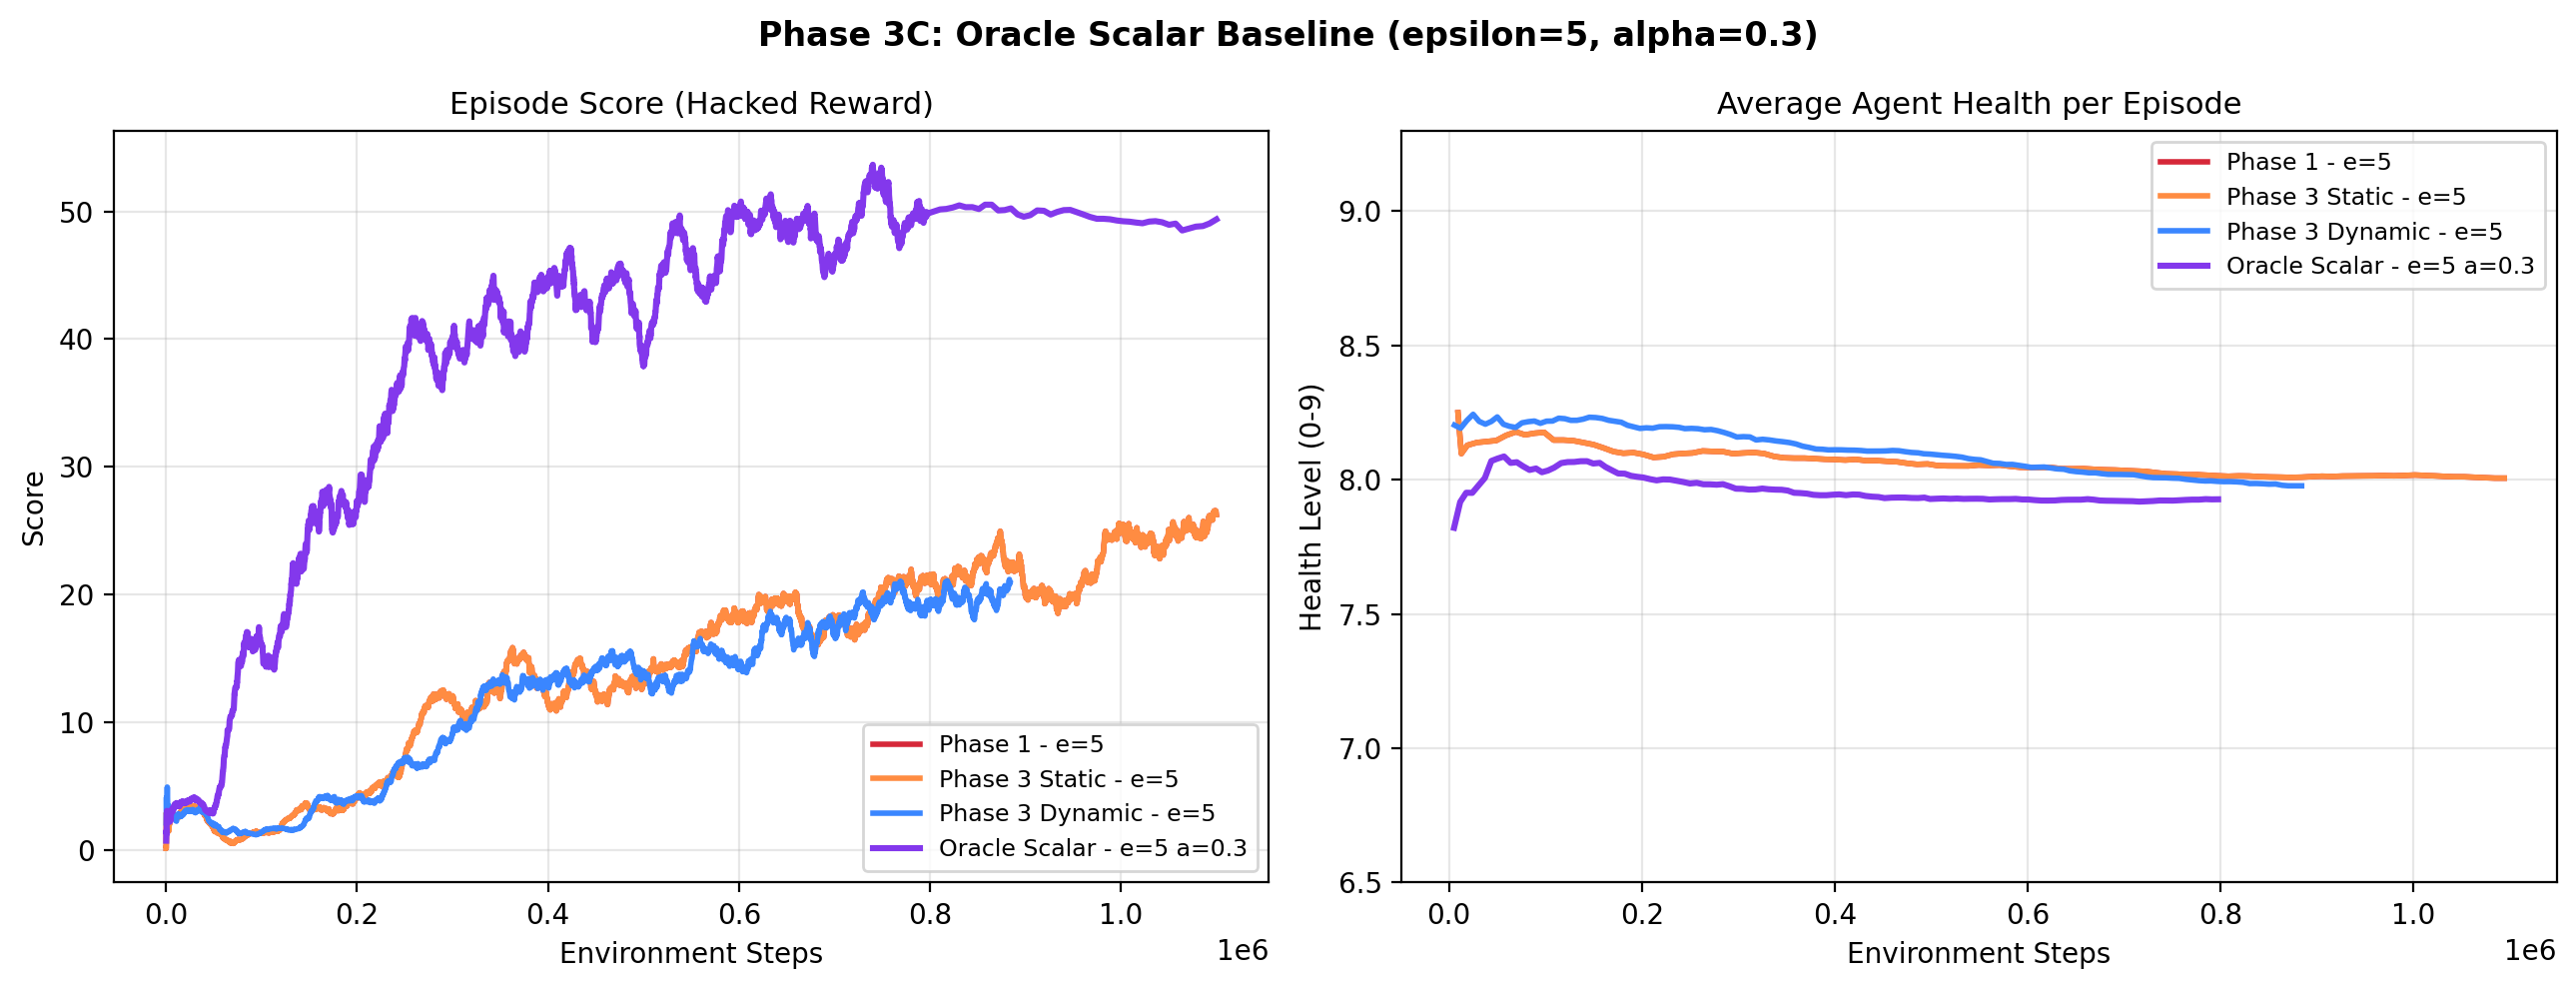
\includegraphics[width=\columnwidth]{fig_phase3_oracle.png}
  \caption{Oracle scalar baseline ($\epsilon=5$, $\alpha=0.3$) vs Phase 1/3 $\epsilon=5$ runs.}
  \label{fig:phase3c_final}
\end{figure}

\begin{figure}[H]
  \centering
  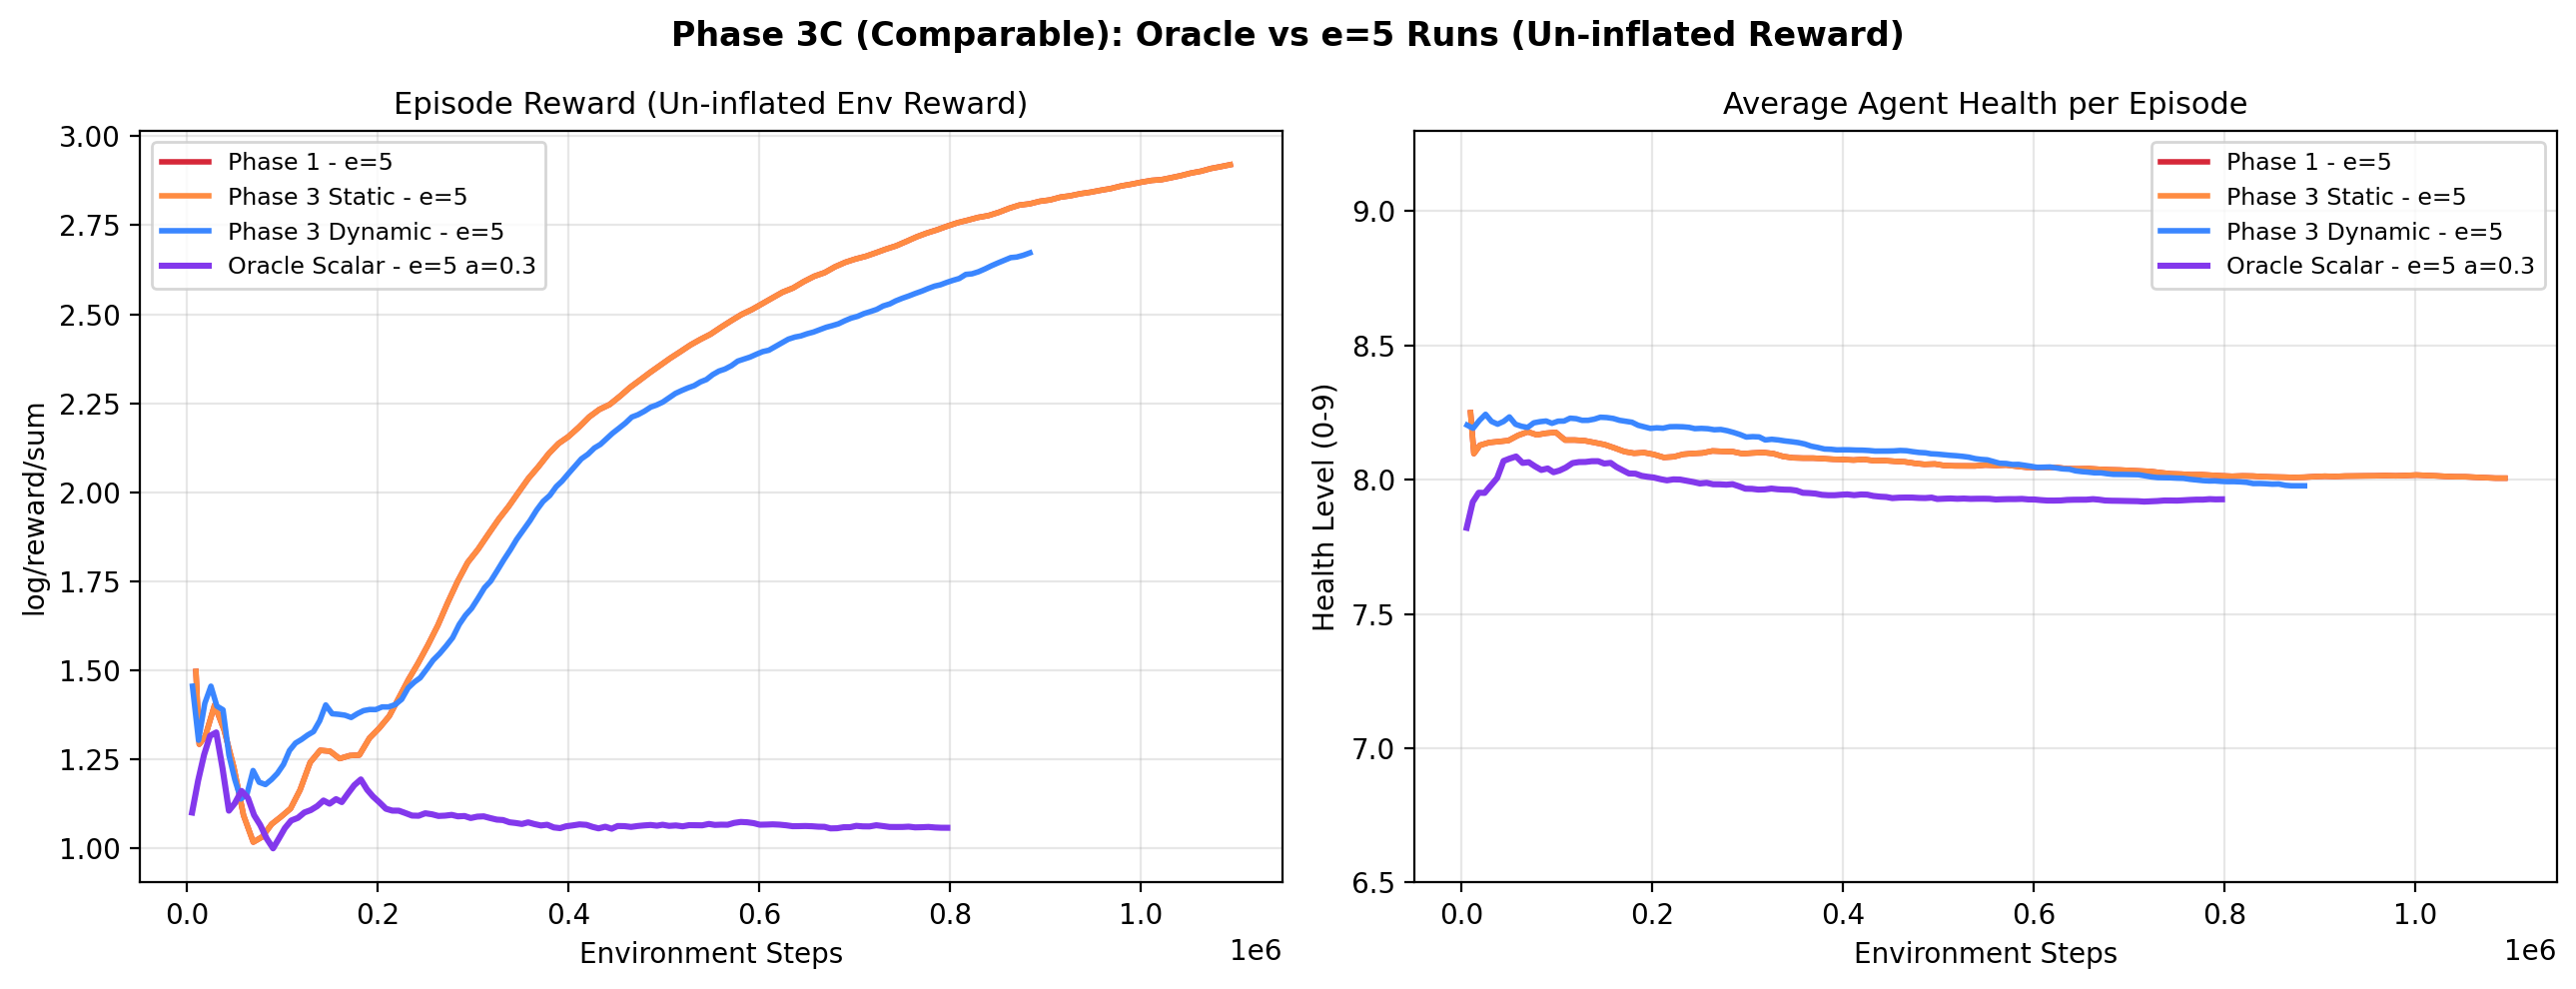
\includegraphics[width=\columnwidth]{fig_phase3_oracle_true_reward.png}
  \caption{$\epsilon=5$ comparison using un-inflated env reward (\texttt{log/reward/sum}).}
  \label{fig:phase3c_true}
\end{figure}

For $\epsilon=5$, oracle training curves extend through merged score logs to \(\sim 1.1\times 10^6\) steps for plotting; metric-derived health/reward panels follow the primary \texttt{metrics} JSONL coverage. Oracle remains competitive with MO variants on several slices but is still a single scalar objective---it does not enforce the same structural separation as Cobb--Douglas MO.

\section{Discussion}
\textbf{What is established.} Controlled misspecification reliably changes behavior; mitigation helps, with dynamic MO strongest among completed architecture variants at high $\epsilon$.\\
\textbf{What is newly added.} Preference-corrected scalar oracle runs at $\epsilon\in\{1,5\}$ with $\alpha=0.3$, plus comparable plots using un-inflated env reward.\\
\textbf{Current limitation.} Oracle evidence is one seed per $(\epsilon,\alpha)$ configuration; multi-seed variance is not yet characterized.

\section{Conclusion}
This project demonstrates a reproducible reward-misspecification benchmark in DreamerV3, evaluates architecture-level mitigation (static/dynamic MO), and adds scalar oracle baselines at moderate and strong perturbation for final comparison. Results support a practical conclusion: mitigation strategies substantially improve robustness, but high-magnitude misspecification remains an open challenge and motivates additional seed-level and ablation-level validation.

\begin{thebibliography}{9}
\bibitem{hafner2023dreamerv3} D. Hafner et al. Mastering diverse domains through world models (DreamerV3). \textit{arXiv:2301.04104}, 2023.
\bibitem{hafner2021crafter} D. Hafner. Benchmarking the spectrum of agent capabilities (Crafter). \textit{arXiv:2109.06780}, 2021.
\bibitem{christiano2017rlhf} P. Christiano et al. Deep RL from human preferences. \textit{NeurIPS}, 2017.
\end{thebibliography}

\end{document}
